\documentclass[11pt,a4paper]{article}
\usepackage[utf8]{inputenc}
\usepackage{amsmath}
\usepackage{amsfonts}
\usepackage{amssymb}

\usepackage[table]{xcolor}

\usepackage{graphicx}
\usepackage{float}

\usepackage[german]{babel}

\usepackage[backend=biber, citestyle=authoryear]{biblatex}

\addbibresource{Sources.bib}

\usepackage[left=3cm, right=3cm, top=3cm, bottom=3cm]{geometry}
\numberwithin{equation}{subsection}

\author{David Bailey}
\title{Versuchsprotokoll 2-3}

\linespread{1.1}

\begin{document}
\selectlanguage{german}

\begin{titlepage}
	\centering
	{Leibniz Universität Hannover\par}
	{\large Grundlagenlabor II\par}	

	\vspace{4.5cm}	
	
	{\huge \bf Versuch 2-3 \par}
	{\Huge \bf Leistung im Wechselstrom\par}
	\vspace{0.3cm}
	
	\vspace{1.5cm}
	
	{\Large David Bailey\par}

	\vfill

	\raggedright

{\Large
\begin{tabular}{ll}
Matrikelnummer:& 10011830 \\
E-Mail: & davidbailey.2889@gmail.com \\
Gruppennummer:& 218 \\
Versuch durchgeführt:& 11.12.2018 \\
Abgabe des Berichtes:& 25.12.2018
\end{tabular}\par}

\end{titlepage}


\tableofcontents

\newpage

\section{Einleitung}

Der in diesem Protokoll beschriebene Versuch \textit{Leistung bei Wechselstrom} befasst sich mit dem Problem der Leistung von periodisch bzw. harmonisch erregten Netzwerken. Es wird auf die verschiedenen Arten von Leistung sowie deren technische Relevanz eingegangen, und verschiedene Methoden der Bestimmung, Berechnung und Darstellung der Leistung werden genauer untersucht.

\subsection{Leistung bei harmonischer Erregung}

Die Grundlage der Leistungsberechnung stellt die Leistung bei harmonischer Erregung dar. Sie beschreibt für ein gegebenes lineares Netzwerk mit sinusförmigen Strömen und Spannungen die abgegebene oder aufgenommene Leistung mithilfe der komplexen Wechselstromrechnung.\\
\\
Für den Fall von $f=0$, d.h. bei einer Erregung mit Gleichstrom, ist bekannt das gilt:
\begin{align*}
P=U\cdot I
\end{align*}
\\
Liegt jedoch eine harmonische Erregung vor, so gilt der obige Term nicht mehr. Strom und Spannung sind nun zeitlich abhängig und können phasenverschoben sein, weshalb man den Zeitpunkt $t$ mit in die Formel aufnehmen muss. Es ergibt sich so der Term der \textit{Momentanleistung}:
\begin{equation} \label{eq:Momentanleistung}
p(t)=u(t)\cdot i(t)
\end{equation}
\\
Dieser gilt nun für alle Arten von Erregung und Belastung. Im Falle der harmonischen Erregung eines Verbrauchers mit den Größen:
\begin{align*}
u(t) &= \hat{U}\sin(\omega t + \varphi_u)\\
i(t) &= \hat{I}\sin(\omega t + \varphi_i)
\end{align*}
lässt sich Formel \eqref{eq:Momentanleistung} schreiben als:
\begin{eqnarray}
&p(t)=&\hat{U}\sin(\omega t + \varphi_u) \cdot \hat{I}\sin(\omega t + \varphi_i) \nonumber \\
\Leftrightarrow & p(t) =&\frac{\hat{U}\hat{I}}{2}\left[\underbrace{\cos(\varphi_u-\varphi_i)[1-\cos(2(\omega t + \varphi_u))]}_{p_w(t)}-\underbrace{\sin(\varphi_u-\varphi_i)\cdot\sin(2(\omega t + \varphi_u))}_{p_B(t)}\right] \label{eq:MomLeistungSplit}
\end{eqnarray}

Bei genauerer Betrachtung von Formel \eqref{eq:MomLeistungSplit} wird festgestellt:
\begin{enumerate}
\item Der Term der Leistung hat die doppelte Frequenz der ursprünglichen Erregung, erkennbar an $\cos(\mathbf{2\omega t} + 2\varphi_u)$ bzw. $\sin(\mathbf{2\omega t} + 2\varphi_u)$.

\item Der Durchschnitt der Leistung liegt nicht bei 0, es wird im Durschnitt eine Leistung, die sog. Wirkleistung, aufgenommen. Sie entspricht:
\begin{equation}
P = \frac{\hat{U}\hat{I}}{2}\cos(\varphi_u-\varphi_i) \label{eq:LeistungGleichanteil}
\end{equation}

\item Es gibt einen um $\frac{\pi}{2}$ zu dieser Gleichanteil-verursachenden Schwingung versetzte Leistung, welche im Durchschnitt keinen Beitrag zur aufgenommenen Leistung beiträgt. Diese als Blindleistung "Q" bezeichnete Leistung hat eine Amplitude von:
\begin{equation}
Q = \frac{\hat{U}\hat{I}}{2}\sin(\varphi_u - \varphi_i) \label{eq:LeistungBlindanteil}
\end{equation}
\end{enumerate}

Die durch Gleichung \eqref{eq:LeistungGleichanteil} angegebene Wirkleistung ist die in der Maschine tatsächlich umgesetzte elektrische Leistung, die durch Gleichung \eqref{eq:LeistungBlindanteil} angegebene Blindleistung wird periodisch von der Maschine aufgenommen und wieder abgegeben, und stellt somit einen unerwünschten Energieaustausch dar.

Die \textit{Scheinleistung} ist die Amplitude der Momentanleistung. Da Blind- und Wirkleistung exakt $\frac{\pi}{2}$ zueinander versetzt sind, lässt sie sich berechnen als:
\begin{equation}
S^2=P^2 + Q^2 = \left(\frac{\hat{U}\hat{I}}{2}\right)^2\cdot \underbrace{(\cos(\varphi_u - \varphi_i)^2 + \sin(\varphi_u - \varphi_i)^2)}_{1}
\end{equation}

Die obigen Formeln lassen sich auch mit der Komplexen Wechselstromrechnung ausdrücken. Diese kodiert den Phasenwinkel von Strom und Spannung im Argument der komplexen Zahl, während die Amplitude der Schwingungen im Betrag zu finden ist. Man kann so also auch schreiben:
\begin{equation}
\underline{S} = \underline{U}\cdot\underline{I}^* = UI\cdot e^{i(\varphi_u-\varphi_i)} \label{eq:KomplexS}
\end{equation}

Gleichungen \eqref{eq:LeistungGleichanteil} und \eqref{eq:LeistungBlindanteil} können nun auch mit der komplexen Scheinleistung ausgedrückt werden:
\begin{eqnarray*}
P=& \mbox{real}(\underline{S}) = UI\cdot \cos(\varphi_u-\varphi_i)\\
Q=& \mbox{img}(\underline{S}) = UI\cdot \sin(\varphi_u-\varphi_i)
\end{eqnarray*}

\subsection{Leistung bei periodischer Erregung}
Liegt ein lineares Netzwerk mit nicht-harmonischer Erregung vor, oder wird ein nichtlineares Bauteil verwendet, so liegen an einem Verbraucher-Zweipol keine harmonischen Ströme und Spannungen mehr an. Dementsprechend können die obigen Formeln nicht mehr angewendet werden. Insbesondere gelten Formeln \eqref{eq:LeistungGleichanteil} und \eqref{eq:LeistungBlindanteil} für Wirk- und Blindleistung nicht mehr.

Durch Verfahren wie der Fourier-Transformation der am Verbraucher gemessenen Ströme und Spannungen kann jedoch auch eine Formel der Momentanleistung berechnet werden. Setzt man die Fourier-Transformierten Ströme und Spannungen in Gleichung \eqref{eq:Momentanleistung} ein, so erhält man:
\begin{equation*}
p(t)=u(t)\cdot i(t) = \sum\sum\left(I_\nu\sin(\nu \omega t+ \varphi_{i\nu})\right) \cdot \left(U_\mu\sin(\mu \omega t + \varphi_{u\mu})\right)
\end{equation*}

Durch ähnliche trigonometrische Umformungen wie für Gleichung \eqref{eq:MomLeistungSplit} verwendet wurden, erhält man:
\begin{equation}
p_{\mu\nu}(t)=\frac{\hat{U}_\mu\hat{I}_\nu}{2}\left[\cos((\mu-\nu)\omega t + (\varphi_{u\mu}-\varphi_{i\nu}))-\cos((\mu+\nu)\omega t + (\varphi_{u\mu}-\varphi_{i\nu}))\right]
\end{equation}

Aus dieser Gleichung kann man erkennen, dass nur Oberwellen gleicher Frequenz einen Gleichanteil, und somit Wirkleistung, beitragen können. Alle anderen Kombinationen schwingen immer um 0, und tragen somit nur zur Blindleistung bei.

Die Wirkleistung eines nicht-harmonischen bzw. nichtliearen Systemes lässt sich somit berechnen als:
\begin{equation}
P_{ges}=\sum_{\mu = 1}^mP_{\mu=\nu}=\sum_{\mu = 1}^m\frac{\hat{U}_\mu\hat{I}_\mu}{2}\cos(\varphi_{u\mu}-\varphi_{i\mu})
\end{equation}

\subsection{Leistungsmessung}
Die Messung der Leistung eines elektrischen Verbrauchers ist eine in der Praxis sehr wichtige Aufgabe, so z.B. um den Stromverbrauch von Geräten zu bestimmen. Es sollen hier also zwei im späteren Versuchsverlauf genutzte Wege der (Wirk)Leistungsbestimmung genauer erläutert werden.

\subsubsection{Darstellung der Leistung}
Um die Phasenverschiebung der harmonischen Leistung bzw. die Form der periodischen Leistung bei nicht-harmonischer Erregung genauer betrachten zu können ist es oft nötig, die $p(t)$-Kurve dar zu stellen. Da fast immer mit Frequenzen von einigen zehn bis hundert Herz gearbeitet wird, lassen sich normale Multimeter nicht mehr verwenden.

Trägheitsarme Anzeigegeräte wie Logikanalysatoren oder Oszilloskope lassen sich jedoch gut verwenden, da sie analoge Signale bis zu einigen tausend Herz anzeigen können. Da sie meist nur Spannungseingänge besitzen, wird der zu messende Strom über einen möglichst geringen Widerstand geleitet, und die dort abfallende Spannung gemessen. So lässt sich die Phasenverschiebung zwischen Strom und Spannung ablesen, aber auch der genaue Verlauf bei einer nichtlinearen Belastung.

Oszilloskope besitzen zusätzlich eine Funktion zum Multiplizieren der Spannungsverläufe. So lässt sich eine zur Leistung proportionale Kurve darstellen, an der sich die doppelte Frequenz, Phasenverschiebung und der Gleichanteil ablesen lassen.

\subsubsection{Wirkleistungsmessung}
Ist nur der Betrag der Wirkleistung, nicht aber die genaue Form, Phasenverschiebung oder die Blindleistung von Interesse, so können auch träge Messgeräte, welche den Mittelwert eines hochfrequenten Signals bilden, zusammen mit einem sog. Multiplikator verwendet werden, um die in einem Verbraucher aufgenommene Wirkleistung zu bestimmen. Der Multiplikator kann hierbei entweder dem Messgerät vorgeschaltet sein, oder aber im Messgerät selbst durch mechanische Verfahren eingebaut sein.

Wird an den Eingängen des Multiplikators nun die am Verbraucher anliegende Spannung und die über einen Messwiderstand abfallende, zum Strom proportionale Spannung, angelegt, so bildet dieser nun nach Gleichung \eqref{eq:Momentanleistung} einen zur Momentanleistung proportionalen Wert. Wird dieser an ein träges Messgerät angeschlossen, so bildet dieses bei höheren Frequenzen den Durchschnitt der Momentanleistung, d.h. nach Gleichung \eqref{eq:MomLeistungSplit} einen zur Wirkleistung proportionalen Wert. Durch Bestimmung der Proportionalitätskonstante kann nun aus dem Ausschlag des Messgerätes die Wirkleistung abgelesen werden.

\subsubsection{Blindleistungsmessung}
Es lässt sich auch die Blindleistung mit einem zur Wirkleistungsmessung ähnlichem Aufbau messen. Da, angegeben von Gleichung \eqref{eq:MomLeistungSplit} die Blindleistung um $\frac{\pi}{2}$ von der Wirkleistung phasenverschoben ist, kann sie durch Phasenverschiebung der Spannung relativ zum Strom gemessen werden.
Durch Einbau eines passend gewählten Kondensators, etwa $\frac{1}{\omega C} = 10R_i$, wird diese Phasenverschiebung der gemessenen Spannung erreicht. Durch den zusätzlichen Widerstand jedoch verringert sich auch die Amplitude der gemessenen Spannung, und somit auch die der Momentanleistung. Dies muss in der Proportionalitätskonstante mit beachtet werden.

\section{Versuchsdurchführung und Auswertung}
\subsection{Messung der Momentanleistung}
\label{sec:Versuch2.2.1}
Dieser Versuchsteil befasst sich mit der grafischen Darstellung der Momentanleistung mithilfe eines Oszilloskopes. Der Verlauf von Strom und Spannung, deren Phasenverschiebung zueinander, und der Zusammenhang zum Verlauf der Momentanleistung wird betrachtet.


\subsubsection{Versuchsaufbau}
\label{sec:Aufbau2.2.1}

Abbildung \ref{fig:Plan2-1} zeigt den in diesem Versuchsteil verwendeten Schaltplan. Folgende Parameter werden verwendet:
\begin{itemize}
\item $Z_1 = \frac{1}{j\omega C} \mbox{ mit } C=4\mu F$
\item $Z_2 = 60\Omega$
\item $Z_3 = R_{sp} + j\omega L$ mit $R_{sp} = 5,5\Omega; L=15,84mH$
\item $u_{ges}$ wird durch Veränderung von $R_I$ auf 6V eingestellt.
\end{itemize}

\begin{figure}[h]
\centering
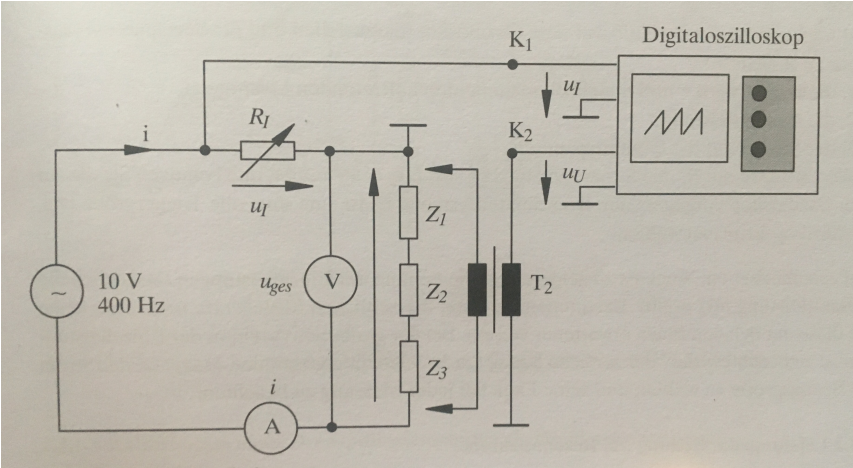
\includegraphics[width=0.7\linewidth]{Images/Aufbau2-1.png}
\caption{Schaltplan Versuch 2.1}
\label{fig:Plan2-1}
\end{figure}
\large{REFERENCE}

Im Folgenden wird das Oszilloskop zur Anzeige der Momentanleistung verwendet. Hierfür wird die Spannung über einen beliebigen Verbraucher mithilfe des potentialtrennenden Transformators $T_2$ am Oszilloskopeingang gemessen. Der Strom $i$ wird anhand der am Widerstand $R_I$ abfallenden Spannung gemessen. Zusätzlich lässt sich der Effektivwert des Stromes am Ampermeter ablesen.

Das Oszilloskop nun wird so eingestellt, dass das Produkt aus $u_I$ und $u_U$ angezeigt wird. Da $u_I$ proportional zu $i$ ist, wird so eine zur Momentanleistung proportionale Kurve angezeigt.

\subsubsection{Momentanleistungskurven}

Die im Folgenden dargestellten Kurven werden vom Oszilloskop abgespeichert. \textit{Ch~1} (blaue Kurve) stellt hierbei die zum Strom proportionale Kurve dar, \textit{Ch~2} (rote Kurve) die am Verbraucher gemessene Spannung. Die Momentanleistung $p(t)$ wird durch die grüne Kurve dargestellt.
\\
Folgende Kurven werden gemessen:

\paragraph{Momentanleistung am Kondensator}
Sie ist in Abbildung \ref{fig:MomLKurveZ1} dargestellt. Deutlich zu sehen ist die Phasenverschiebung von Strom und Spannung, welche bei ca. $\frac{\pi}{2}$ liegt. Die Kurve der Momentanleistung schwingt mit doppelter Frequenz um 0, besitzt also keinen Gleichanteil. Dies entspricht genau der Vorhersage von Gleichung \eqref{eq:MomLeistungSplit} bzw. \eqref{eq:LeistungGleichanteil}, welche für eine Phasenverschiebung von $\varphi_u - \varphi_i = -\frac{\pi}{2}$, wie sie beim Kondensator vor liegt, eine rein sinusförmige Schwingung und keine Wirkleistung vorhersagen. Der Kondensator nimmt somit entsprechend Gleichung \eqref{eq:KomplexS} eine Leistung von $\underline{S} = UIe^{-i\frac{\pi}{2}}$ auf.\par

\begin{figure}[H]
\centering
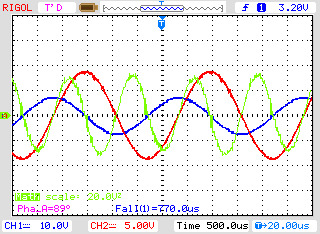
\includegraphics[width=0.7\linewidth]{Oszi-Bitmaps/NewFile0.jpg}
\caption{Momentanleistung am Kondensator. $u_I(t)$ (Blau), $u_{Z1}(t)$ (Rot), $p_{Z_1}(t)$ (Grün)}
\label{fig:MomLKurveZ1}
\end{figure}

\paragraph{Momentanleistung am Ohm'schen Widerstand}
Die Kurve der an einem Ohm'schen Widerstand gemessenen Momentanleistung ist in Abbildung \ref{fig:MomLKurveZ2} zu sehen. Da es sich um einen Verbraucher mit rein realer Impedanz handelt, gibt es keine Phasenverschiebung zwischen $u(t)$ und $i(t)$. Dies ist deutlich in der Grafik zu erkennen. Entsprechend Gleichung \eqref{eq:MomLeistungSplit} sollte die Kurve der Momentanleistung für $\varphi_u = \varphi_i$ rein positiv sein, und einen deutlichen Gleichanteil von $UI$ besitzen. Auch dies ist in der Grafik klar erkennbar. Der Widerstand nimmt also konstant Leistung auf, es wird keine Leistung abgegeben. Entsprechend Gleichungen \eqref{eq:LeistungGleichanteil} und \eqref{eq:LeistungBlindanteil} ist die Wirkleistung maximal, die Blindleistung minimal.


\begin{figure}[H]
\centering
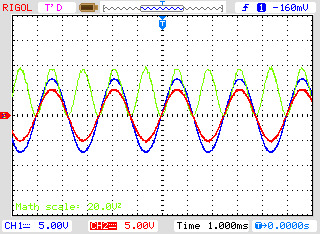
\includegraphics[width=0.7\linewidth]{Oszi-Bitmaps/NewFile1.jpg}
\caption{Momentanleistung am Ohm'schen Widerstand. $u_I(t)$ (Blau), $u_{Z2}(t)$ (Rot), $p_{Z_2}(t)$ (Grün)}
\label{fig:MomLKurveZ2}
\end{figure}

\paragraph{Momentanleistung an einer Spule}
Die Kurve der an einer Spule mit nicht-vernachlässigbarem Innenwiderstand ($R_{sp} = 5\Omega)$ ist in Abbildung \ref{fig:MomLKurveZ3} zu sehen. Ähnlich wie beim Kondensator (Abbildung \ref{fig:MomLKurveZ1}) ist eine Phasenverschiebung zwischen Strom und Spannung zu sehen. Diese ist jedoch etwas kleiner als die für eine reine Induktivität erwarteten $\frac{\pi}{2}$, welches sich durch den Innenwiderstand erklären lässt. Durch eine Komplexe Impedanz von $\underline{Z} = R_{sp} + j\omega L = 5,5\Omega + j39,81\Omega$ lässt sich eine Phasenverschiebung von $arc(\underline{Z}) = 82,134^\circ$ erwarten. Dies stimmt in etwa mit der Messung des Oszilloskopes überein. Entsprechend Gleichung \eqref{eq:MomLeistungSplit} sollte die Kurve der Momentanleistung einen kleinen Gleichanteil von etwa $P = \cos(\varphi)*S=0.136*S$ besitzen. Auch dies lässt sich in der Abbildung erkennen. Dennoch überwiegt entsprechend Gleichung \eqref{eq:LeistungBlindanteil} die Blindleistung der Spule mit $Q=\sin(\varphi)*S=0.99*S$

\begin{figure}[H]
\centering
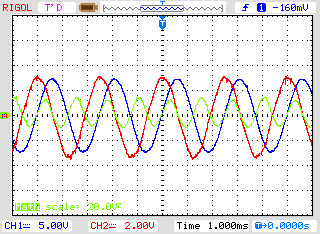
\includegraphics[width=0.7\linewidth]{Oszi-Bitmaps/NewFile2.jpg}
\caption{Momentanleistung an einer Spule mit Innenwiderstand. $u_I(t)$ (Blau), $u_{Z3}(t)$ (Rot), $p_{Z_3}(t)$ (Grün)}
\label{fig:MomLKurveZ3}
\end{figure}

\paragraph{Momentanleistung der gesamten Schaltung}
Die Kurve der in der gesamten Schaltung verbrauchten Momentanleistung ist in Abbildung \ref{fig:MomLKurveGesamt} zu erkennen. Da es sich hier um eine beliebig zusammengesetzte komplexe Impedanz handelt, lässt sich direkt keine Vorhersage über den Verlauf der Momentanleistung formulieren. Der hohe Gleichanteil legt jedoch nahe, dass die am Widerstand abfallende Leistung überwiegt. Die Phasenverschiebung lässt sich aus der Grafik als $\varphi = -\frac{\pi}{4}$ ablesen, und stimmt der obigen Vermutung zu.
Durch Summierung der Impedanzen der Komponenten lässt sich die Gesamtimpedanz berechnen:
\begin{eqnarray*}
\underline{Z}_{ges} =& \sum_{\mu=1}^3\underline{Z}_\mu = 65.5\Omega - j59.66\Omega\\
\mbox{Arg}(\underline{Z}) =& -42.33^\circ
\end{eqnarray*}
Die berechnete Phasenverschiebung entspricht hier also fast genau der anhand der Abbildung geschätzten.

Entsprechend Gleichungen \eqref{eq:LeistungGleichanteil} und \eqref{eq:LeistungBlindanteil} ist es also tatsächlich so, dass Blind- und Scheinleistung hier etwa den gleichen Betrag von $\sin(45^\circ)*S=\cos(45^\circ)*S = \frac{1}{\sqrt{2}} * S$ besitzen.

\begin{figure}[H]
\centering
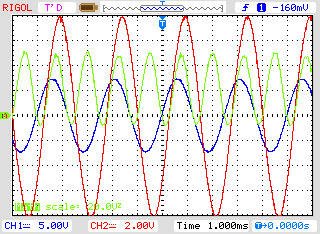
\includegraphics[width=0.7\linewidth]{Oszi-Bitmaps/NewFile3.jpg}
\caption{Momentanleistung der gesamten Schaltung. $u_I(t)$ (Blau), $u_{ges}(t)$ (Rot), $p_{ges}(t)$ (Grün)}
\label{fig:MomLKurveGesamt}
\end{figure}

\subsubsection{Grafische Addition der Leistung}
Es wird nun noch überprüft, ob sich die Momentanleistung der einzelnen Impedanzen addieren lassen, um die Momentanleistung des gesamten Systemes zu erhalten. Hierfür werden für einige beliebig gewählte Phasenwinkel die Werte der Momentanleistung aus den Oszilloskop-Messungen abgelesen, und miteinander verglichen.

\begin{center}
\begin{tabular}{| r | c | c | c | c | c|}
\hline
\multicolumn{6}{|c|}{Tabelle 1: Abgelesene Momentanleistungswerte} \\
\hline
$\varphi$ & $p_{Z_1}$ & $p_{Z_2}$ & $p_{Z_3}$  & $p_{Z_{sum}}$ & $p_{Z_{ges}}$ \\
\hline 
$0^\circ$ & $0V^2$ & $0V^2$ & $0V^2$ & $0V^2$ & $0V^2$ \\
$45^\circ$ & $-30V^2$ & $20V^2$ & $10V^2$ & $0V^2$ & $0V^2$\\
$90^\circ$ & $0V^2$ & $35V^2$ & $0V^2$ & $35V^2$ & $30V^2$ \\
\hline
\end{tabular}
\end{center}

Abgesehen von einer leichten Diskrepanz bei $\varphi = 90^\circ$ welche durch die Ungeauigkeit beim Ablesen erklärt werden kann, gleicht sich die Summe der einzelnen Momentanleistungen mit der im gesamten System verbrauchten Leistung. Dies ist auch mathematisch zu erwarten, da gilt:
\begin{eqnarray*}
& \underline{S}_{ges} =& \underline{U}_{ges}\cdot\underline{I}^* \\
\Leftrightarrow &\underline{S}_{ges} =& \underline{Z}_{ges}\cdot\underline{I}\cdot\underline{I}^* = \underline{Z}_{ges}\cdot |\underline{I}|^2 \\
\Leftrightarrow & \underline{S}_{ges} =& \underbrace{(\underline{Z}_1 + \underline{Z}_2 + \underline{Z}_3)}_{Z_{ges}} \cdot |\underline{I}|^2 \\
\Leftrightarrow & \underline{S}_{ges} =& \sum_{\mu=1}^3 \underbrace{\left(\underline{Z}_\mu \cdot |\underline{I}|^2\right)}_{S_\mu}\\
\end{eqnarray*}

\newpage
\subsection{Leistung im Resonanzfall}

Dieser Versuchsteil befasst sich mit der Messung der Momentanleistung an einem LCR-Schwingkreis, welcher unter Resonanzbedingung betrieben wird. Das Verhalten des Schwingkreises wird genauer untersucht, und der Momentanleistungsverlauf wird erläutert.

\subsubsection{Versuchsaufbau}
Der Aufbau dieses Versuches ist identisch mit dem in Abschnitt \ref{sec:Aufbau2.2.1} verwendeten Aufbau. Einzig die Impedanzen werden verändert. Es gilt nun:
\begin{itemize}
\item $Z_1 = \frac{1}{j\omega C} \mbox{ mit } C=10\mu F $
\item $Z_2 = 40\Omega$
\item $Z_3 = R_{sp} + j\omega L \mbox{ mit } L=15,84mH$
\item $R_i$ wird nicht verändert. 
\end{itemize}

Das Oszilloskop wird weiterhin zur Messung der Momentanleistung über beliebige Verbraucher verwendet, und wird wieder so eingestellt, dass die Momentanleistung als Produkt aus $u_I$ und $u_U$ angezeigt wird. Erneut gilt, dass die angezeigte Kurve nur proprotional zu $p(t)$ ist, da $R_i$, und somit $i(t)$, nicht exakt bekannt sind.

\subsubsection{Momentanleistungskurve}

Wie im in Abschnitt \ref{sec:Versuch2.2.1} erläuert wird die Momentanleistungskurve mit dem Oszilloskop aufgenommen. In Abbildung \ref{fig:MomLKurveResonanz} ist die zum Strom proportionale Kurve $u_I(t)$ in Blau, die Spannungskurve $u_U(t)$ in Rot, und das zur Momentanleistung proportionale Produkt in grün.

\begin{figure}[H]
\centering
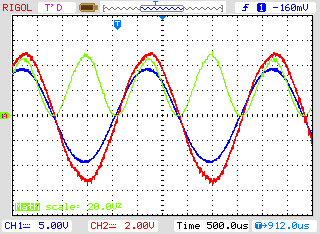
\includegraphics[width=0.7\linewidth]{Oszi-Bitmaps/NewFile4.jpg}
\caption{Momentanleistung eines LCR-Oszillators im Resonanzfall. $u_I(t)$ (Blau), $u_{Z_{ges}}(t)$ (Rot), $p_(t)$ (Grün)}
\label{fig:MomLKurveResonanz}
\end{figure}

Deutlich zu sehen ist die gleiche Phase von Strom und Spannung, und die daraus resultierende, nur positive Momentanleistungskurve. Dies ist entgegen erster Intuition, da sich im Schaltkreis auch Verbraucher mit komplexer Impedanz befinden, welche normalerweise Blindleistung hinzufügen bzw. verbrauchen.
Begründen lässt sich dies jedoch, indem das Zeigerbild der über die einzelnen Verbraucher abfallende Spannung gezeichnet wird. Dieses ist in der Abbildung \ref{fig:ZeigerbildResonanz} zu sehen.

\begin{figure}[H]
\centering
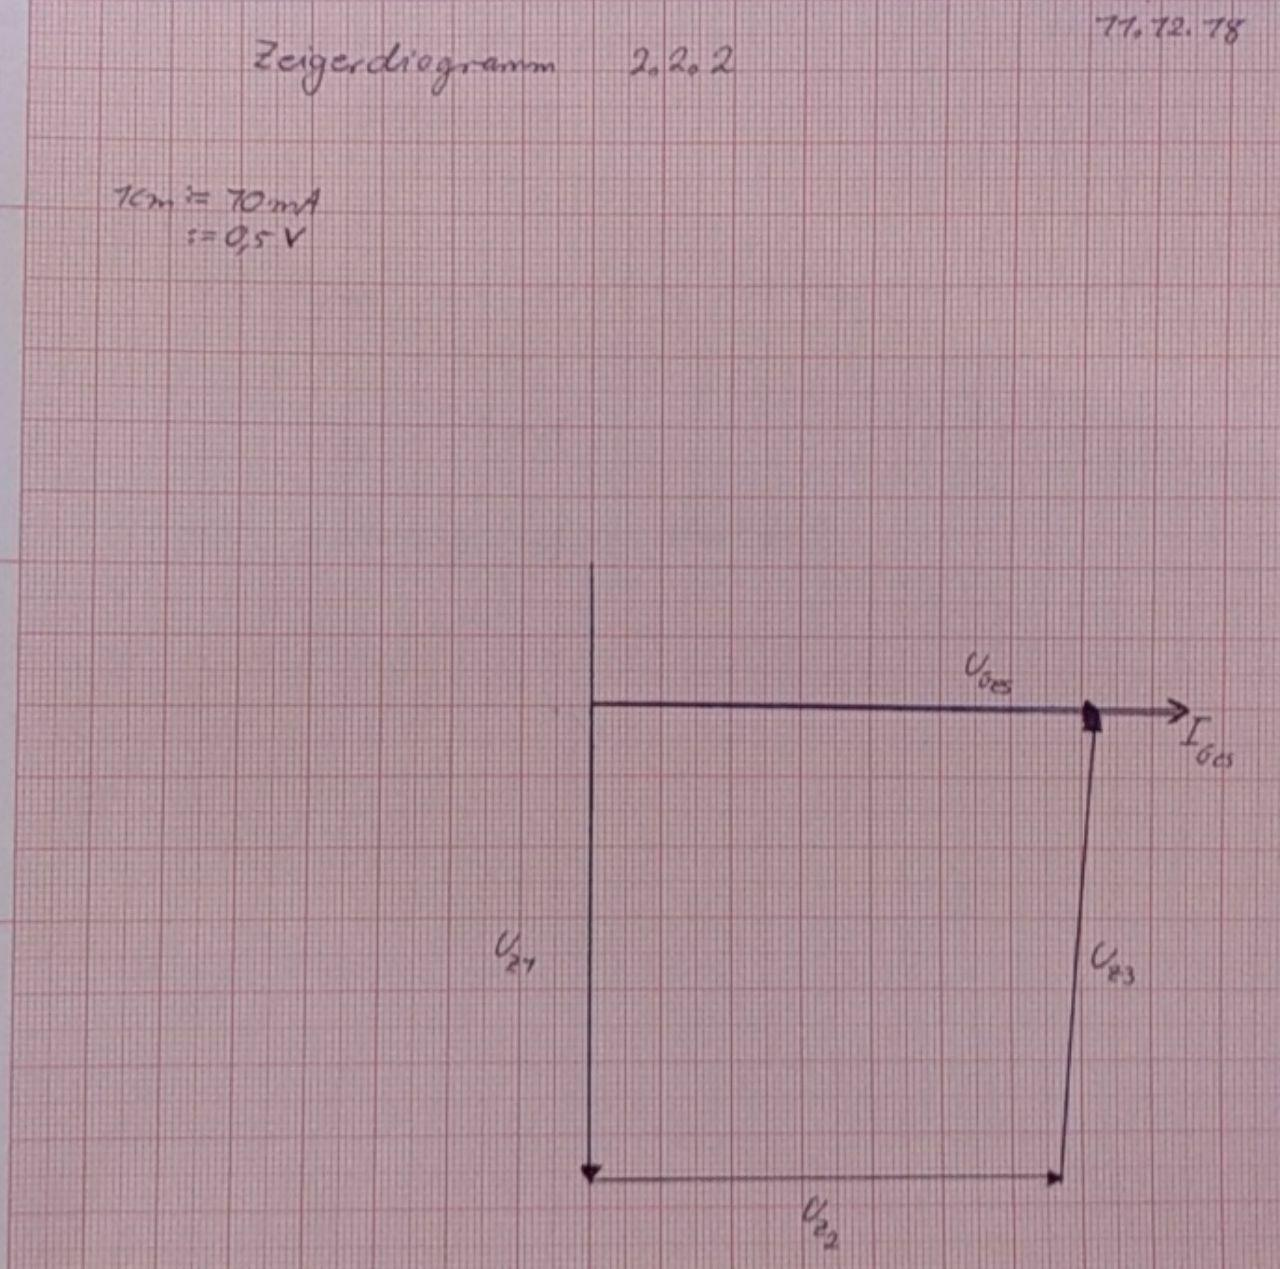
\includegraphics[width=0.7\linewidth]{Images/Zeigerdiagramm2-2-2.jpg}
\caption{Zeigerbild der Spannungen eines LCR-Schwingkreis im Resonanzfall}
\label{fig:ZeigerbildResonanz}
\end{figure}

Erkennbar ist die fast perfekte $180^\circ$ Phasenverschiebung und der gleiche Betrag zwischen $\underline{U}_{Z1}$ und $\underline{U}_{Z3}$, d.h. die Spannungen über Kondensator und Spule. Die zwei Spannungen löschen sich gegenseitig aus, das System verhält sich dementsprechend wie eine rein reelle Impedanz und besitzt keine Phasenverschiebung zwischen $\underline{U}_{ges}$ und $\underline{I}$. Dies ist typisches Verhalten für Schwingkreise im Resonanzfall, und kann bei relativ geringen Innenwiderständen des Verbrauchers zu Schäden führen, sofern der Schaltkreis ungewollt anfängt zu schwingen.

Die komplexe Impedanz diese Schaltkreises beträgt:
\begin{equation*}
\underline{Z}_{ges} = \frac{1}{j\omega C} + R + R_{sp} + j\omega L = 45.5\Omega + j0.021\Omega
\end{equation*}
Wie für einen resonierenden Schwingkreis erwartet verhält er sich von außen wie eine rein reelle Impedanz, der komplexe Teil ist vernachlässigbar klein. Somit nimmt er entsprechend Gleichung \eqref{eq:KomplexS} fast ausschließlich Wirkleistung auf.


\newpage
\subsection{Leistung einer nichtlinearen Belastung}

Dieser Versuch befasst sich mit der an einer Diode, einem nichtlinearem Bauteil, gemessenen Momentanleistung. Es wird kurz auf den Zusammenhang zwischen Strom, Spannung und Momentanleistung eingegangen, und eine vereinfachte Fourier-Transformation wird durchgeführt.

\subsubsection{Versuchsaufbau}
Der Versuchsaufbau ähnelt weitestgehend dem in Abschnitt \ref{sec:Aufbau2.2.1} beschriebenen. Die Verbraucher werden jedoch ersetzt durch eine Diode sowie einem Vorwiderstand von $R_V=50\Omega$. $u_I(t)$ und $u_U$ werden weiterhin im Oszilloskop zu einer zu $p(t)$ proportionalen Kurve multipliziert.
$R_I$ wird so eingestellt, dass das Spannungsmessgerät $u_{ges} = u_{max} = 9V$ anzeigt.

\subsubsection{Auswertung der Momentanleistungskurve}

Wie in Abschnitt \ref{sec:Versuch2.2.1} erläutert wird die Momentanleistungskurve mit dem Oszilloskop aufgenommen. Sie ist in Abbildung \ref{fig:MomLKurveNichtlinear} zu sehen. $u_U(t)$ ist in Rot, $u_I(t)$ in Blau und das zu $p(t)$ proportionale Produkt der Spannungen ist in Grün zu sehen.

\begin{figure}[H]
\centering
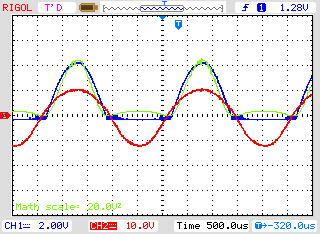
\includegraphics[width=0.8\linewidth]{Oszi-Bitmaps/NewFile5.jpg}
\caption{Momentanleistung einer nichtlinearen Belastung. $u_I(t)$ (Blau), $u_{Z_{ges}}(t)$ (Rot), $p_(t)$ (Grün)}
\label{fig:MomLKurveNichtlinear}
\end{figure}

Deutlich zu sehen ist die nichtlineare Eigenschaft der Diode. In einer Hälfte der Spannungskurve leitet die Diode, die Spannung fällt über dem Widerstand ab und es wird Wirkleistung umgesetzt. In der nächsten Hälfte wird die Diode in Sperrichtung betrieben, es fließt nur noch der Strom des potentialtrennenden Transformators sowie ein kleiner Leckstrom, und ein deutlich geringerer Anteil an Wirkleistung wird umgesetzt. Auch der Spannungsabfall der Diode in Durchlassrichtung ist zu erkennen. Strom beginnt erst ab einer gewissen Spannung zu fließen.
Zu sehen ist auch, dass die Diode sich nicht wie eine komplexe Impedanz verhält. Strom und Spannung sind nicht phasenverschoben und die Kurve der Momentanleistung ist ausschließlich positiv, von der Schaltung wird nie Leistung abgegeben. Zu bemerken ist auch, dass die Momentanleistung nun die gleiche Frequenz wie die Erregerfrequenz besitzt.

Im folgenden werden einige der gemessenen Effekte vernachlässigt, um die Fourier-Analyse in einem verständlichen Umfang zu behalten. Vor allem der Leckstrom wird ignoriert, und es wird von einer perfekten Diode mit 0V Spannungsabfall ausgegangen. 
Eine erste Abschätzung der umgesetzten Leistung ergibt sich zu:
\begin{equation}
P = \frac{1}{2} UI = \frac{1}{4}\hat{U}\hat{I}
\end{equation}
Grund dafür ist, dass sich die Schaltung für eine halbe Periode wie ein ohm'scher Verbraucher verhält, die nächste halbe Periode jedoch wie ein offener Schaltkreis.
Zur Vereinfachung der Fourier-Analyse wird angenommen, dass die Funktion des Stromes wie folgt definiert ist:
\begin{equation}
i(t)=\hat{I}\cdot \left\{ 
\begin{array}{ccr}
	sin(\omega t) & \mbox{for} & kT < t \leq (k+\frac{1}{2})T \\
	0 & \mbox{for} & (k+\frac{1}{2})T < t \leq (k+1)T
\end{array}
\right.
\end{equation}
[\cite{calpolyFourier}]

Anhand eines Tabellenbuches für Fourier-Transformationen lässt sich ablesen, dass sich $i(t)$ mit folgender Reihe annähern lässt:
\begin{equation}
i(t) = \frac{\hat{I}}{\pi} + \frac{\hat{I}}{2}\sin(\omega t) - \frac{2\hat{I}}{\pi}\sum_{n=1}^{\infty}\frac{\cos(2n\omega t)}{4n^2 - 1}
\end{equation}
Die Spannung wird weiterhin als sinusförmige Spannung der Frequenz $\omega$ betrachtet.

Soll nun die Wirkleistung anhand von Formel \eqref{eq:WirkleistungFourier} berechnet werden, so fallen einige Terme weg. Es gilt insbesondere, dass alle geraden Oberwellen eine Phasenverschiebung von $\varphi_{i\mu} = 90^\circ$ besitzen, alle ungeraden Oberwellen eine Amplitude von 0. Eingesetzt in Gleichung \eqref{eq:WirkleistungFourier} ergibt dies:
\begin{equation}
P_{ges} = \sum_{\mu=1}^m\frac{\hat{U}\hat{I_\mu}}{2}\cos(-\varphi_{i\mu})
\end{equation}

Es fallen also alle Terme bis auf die Grundschwingung weg. Diese besitzt eine Amplitude von $\hat{I}_{1}=\frac{\hat{I}}{2}$. Eingesetzt in die obige Gleichung ergibt sich:

\begin{equation}
P_{ges} = \frac{\hat{U}\hat{I}}{4}
\end{equation}
Dies stimmt exakt mit der obigen Vermutung überein. Die Schaltung aus Diode und Widerstand nimmt also in etwa die Hälfte der Leistung eines reinen Widerstandes gleicher Größe auf.

\newpage

\subsection{Leistungsmessung}
Dieser Versuch befasst sich mit der Messung der Wirk- und Blindleistung mithilfe eines Multiplikators und eines trägen Messgerätes. Es wird zusätzlich die Scheinleistung berechnet und die berechneten und gemessenen Ergebnisse werden miteinander verglichen.

\subsubsection{Versuchsaufbau}

Der Versuchsaufbau ähnelt weitestgehend dem in Abschnitt \ref{sec:Aufbau2.2.1} beschriebenen Aufbau. Es wird jedoch das Oszilloskop durch einen Multiplikator und ein träges, analoges Messgerät gemäß Abbildung \ref{fig:Plan2-2} ersetzt. Das Messgerät wird auf Gleichspannung eingestellt und misst somit den Gleichanteil der Spannung $u_P(t)$, welche durch die Multiplikation von Spannung $u_U(t)$ und zum Strom proportionalen Spannung $u_I(t)$ eine zur Momentanleistung proportionale Größe darstellt. Somit kann nach Bestimmung des Proportionalitätsfaktors die Wirkleistung gemessen werden.

\begin{figure}[H]
\centering
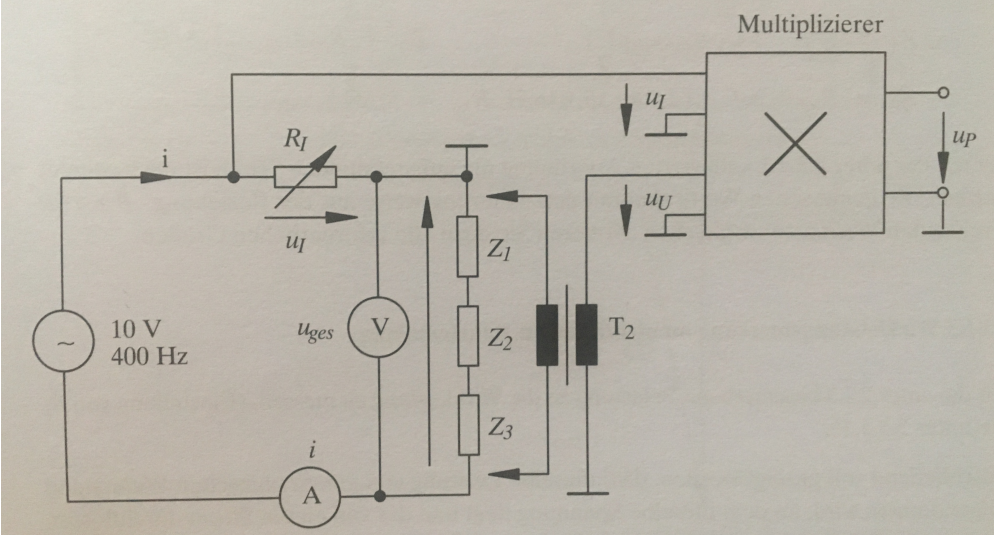
\includegraphics[width=0.7\linewidth]{Images/Aufbau2-2.png}
\caption{Schaltplan eines Versuches zur Messung der Wirkleistung eines Schaltkreises [\cite[49]{GEMLBuch}]}
\label{fig:Plan2-2}
\end{figure}
Die Impedanzen $Z_1$ bis $Z_3$ werden je nach zu messender Größe verändert.

\subsubsection{Kalibrierung des Drehspulmessinstrumentes}
Damit die Wirkleistung aus den am Messgerät abgelesenen Werten errechnet werden kann, muss die Proportionalitätskonstante, im Folgenden "K", sowie der Offset des Multiplizierers bestimmt werden.
Es gilt:
\begin{equation}
K\cdot \overline{u_P(t)} = P
\label{eq:PropFaktor}
\end{equation}

Der Offset wird gemessen indem die Anschlüsse des potentialtrennenden Transformators kurzgeschlossen werden. $u_U(t)=0$ gilt nun, d.h. das Messgerät sollte null anzeigen.
Angezeigt wird jedoch ein Wert von $-1mV$, d.h. die gemessenen Werte müssen um $1mV$ korrigiert werden. Alle im Folgenden aufgeführten Messwerte wurden um diesen Faktor bereits korrigiert.

Es wird $Z_1 = 40\Omega; Z_2 = Z_3 = 0\Omega$ eingebaut. $u_{ges}$ wird durch Veränderung von $R_I$ auf 6V eingestellt. $I$ wird hierbei als $0.16A$ gemessen. Durch eine Phasenverschiebung von $\varphi = 0$ am ohm'schen Verbraucher lässt sich nun die Wirkleistung entsprechend \eqref{eq:LeistungGleichanteil} berechnen als:
\begin{equation*}
P_{mes}=U_{ges}I = 6V\cdot 0.16A = 0.96W
\end{equation*}
Das Messgerät zeigt eine Spannung von $\overline{u_P}=0.475V$ an. 
Durch Umstellen von Gleichung \eqref{eq:PropFaktor} lässt sich nun der Proportionalitätsfaktor bestimmen:
\begin{equation*}
K=\frac{P_{mes}}{\overline{u_P}} = \frac{0.96W}{0.475V} = 2.021A
\end{equation*}

\subsubsection{Messung der Wirkleistung}

Dieser Versuchsteil befasst sich mit der Messung der Wirkleistung, welche von verschiedenen Verbrauchern aufgenommen wird. Der Versuchsaufbau gleicht dem vorherigen Versuchsteil, bis auf die Impedanzen. Für sie gilt nun:
\begin{itemize}
\item $Z_1 = \frac{1}{j\omega C} \mbox{ mit } C = 6\mu F$
\item $Z_2 = [30; 40; \cdots; 80]\Omega$
\item $Z_3 = R_{sp} + j\omega L \mbox{ mit } L = 15.84mH; R_{sp} = 5.5\Omega$
\end{itemize}
$R_I$ darf hierbei nicht mehr verändert werden. Grund dafür ist, dass die Spannung $u_I$, welche zur Berechnung von $u_P$ und somit der Wirkleistung verwendet wird, von $R_I$ abhängt.
Im Folgenden wird $Z_2$ variiert. Die Spannung $\overline{u_P}$ wird abgelesen und mit Gleichung \eqref{eq:PropFaktor} wird die Wirkleistung berechnet. Zusätzlich werden $U_{ges}$ und $I$ an den Messgeräten abgelesen. Zum Vergleich wird die Wirkleistung mit Formel \eqref{eq:KomplexP} und der komplexen Impedanz $Z_{ges}$ berechnet.
\\
Die aufgenommenen Messwerte sind in Tabelle \ref{tab:Wirkleistungen} zu sehen.

Zu erkennen ist eine relativ genaue Übereinstimmung der gemessenen Werte mit den berechneten. Ungenauigkeiten beim Ablesen der analogen Skala am Messgerät erklären die konstanten Werte zwischen $Z_2 = 40\Omega$ und $60\Omega$, weitere Abweichungen von den berechneten Werten können durch Messfehler bei der Bestimmung des Faktors K und dem Offset entstehen. Auch ist es möglich, dass $Z_1 \mbox{ bis } Z_2$ nicht die angegebenen Werte besitzen, d.h. die berechnete Wirkleistung kann auch fehlerbehaftet sein.

\subsubsection{Messung der Blindleistung}
Dieser Versuchsteil befasst sich mit der Messung der Blindleistung der bereits im vorherigen Abschnitt verwendeten Impedanzen. Anhand der Formel \eqref{eq:ScheinleistungPythagoras} werden zusätzlich die Messergebnisse miteinander verglichen.

Um die Blindleistung mit möglichst wenig Aufwand, d.h. hier mit möglichst wenig Modifikation an der vorliegenden Schaltung messen zu können, wird wie in Abschnitt \ref{sec:MessungBlindleistung} erläutert, ein Kondensator in den Spannungspfad des Messgerätes eingebaut, um dessen Phase um $90^\circ$ zu drehen. Hiermit gibt der Gleichanteil der Spannung $u_P$ die Blindleistung, nicht mehr die Wirkleistung, an.

Es wird ein Kondensator von $C=2nF$ direkt hinter $T_2$ geschaltet. Dessen Größe wurde so bemessen, dass eine Phasenverschiebung von ca. $84^\circ$ möglich ist ohne dass das Spannungssignal zu klein wird. $u_U$ ist nun durch die Impedanz des Kondensators etwa 10 mal kleiner, der Kalibrierungsfaktor $K$ muss dementsprechend angepasst werden. Es gilt jetzt:
\begin{equation*}
K_{Q} = 10\cdot K = 20.21A
\end{equation*}

Für die gleichen Impedanzen wie zuvor werden nun die Spannungen $\overline{u_P}$ gemessen und die Blindleistungen berechnet. Gesamtströme und -spannungen sind aus den vorherigen Messungen bekannt. Die anhand von Formel \eqref{eq:KomplexQ} berechnete Blindleistung wird zum Vergleich aufgeschrieben. Die Ergebnisse sind in Tabelle \ref{tab:Blindleistungen} zu sehen.

Auch hier ist eine gute Übereinstimmung der Messwerte mit den berechneten Werten erkennbar. Diskrepanzen lassen sich wie zuvor durch ein falsch bestimmtes K, Ablese- und Messfehler erklären. Einzubeziehen ist auch, dass die Phasenverschiebung nur ca. $84^\circ$ beträgt, und der genaue Wert des Kondensators nicht exakt $2nF$ sein muss.

Schlussendlich lassen sich nun die Messwerte anhand von Formel \eqref{eq:ScheinleistungPythagoras} miteinander vergleichen. $S_1$ wird hierbei mit der Beziehung $S=U\cdot I$ berechnet, $S_2$ anhand von Formel \eqref{eq:ScheinleistungPythagoras}. Die Ergebnisse sind in Tabelle \ref{tab:Scheinleistungen} aufgeführt.

\newpage
\section{Zusammenfassung}

Der Versuch \textit{Leistung im Wechselstrom} erläuterte die verschiedenen Arten der Leistung, welche im Wechselstrom im Vergleich zum Gleichstrom auftreten können. Diese wurden im ersten Versuchsteil anhand einiger Messungen der Momentanleistungen mit einem trägheitsfreien Oszilloskop dargestellt. Die Leistung an verschiedenen Verbrauchern wurde untersucht und die Addierbarkeit der einzelnen Leistungen wurde grafisch und mathematisch bewiesen. Es wurde die Blindleistungskompensation anhand eines LCR-Schwingkreises in Resonanz erläutert. Zusätzlich wurde die Leistung einer nichtlinearen Belastung betrachtet, und eine simple Fourier-Analyse der Leistung durchgeführt.

Im zweiten Versuchsteil wurden die Wirk-, Blind- und Scheinleistungen verschiedener Belastungen mit trägen, mittelwertsbildenden Messgeräten aufgenommen. Die Funktionsweise der jeweiligen Messchaltung wurde erläutert, und die gemessenen und berechneten Werte wurden miteinander verglichen. Unstimmigkeiten der gemessenen Werte wurden auf passende Fehlerquellen zurückgeführt. Schlussendlich wurde die Scheinleistung der jeweiligen Belastung auf verschiedene Arten berechnet, und die Werte wurden miteinander verglichen.

\newpage

\setcounter{section}{0}
\renewcommand{\thesection}{\Alph{section}}
\section{Literaturverzeichnis}
\printbibliography
\newpage
\rowcolors{1}{lightgray}{white}

\section{Verwendete Geräte}

\begin{table}[H]
\begin{center}
\begin{Large}
\begin{tabular}{| l | r |}
\hline
1 Zweikanaloszilloskop & QX 168\\
1 Schaltungstableu & ST 27\\
1 Vielfachmessinstrument & IU 177 + IU 30\\
1 Variabler Kondensator & CG 69\\
1 Variabler Widerstand & RG 239
\end{tabular}
\end{Large}
\end{center}
\end{table}

\section{Tabellen}

\begin{table}[H]
\caption{Am Oszilloskop abgelesene Messwerte zur grafischen Addition der Leistung}
\label{tab:Momentanleistungswerte}
\begin{center}
\begin{Large}
\begin{tabular}{| r | c | c | c | c | c|}
\hline
\rowcolor{blue}\color{white} $\varphi$ & \color{white}$p_{Z_1}$ & \color{white}$p_{Z_2}$ & \color{white}$p_{Z_3}$  & \color{white}$p_{Z_{sum}}$ & \color{white}$p_{Z_{ges}}$ \\
\hline 
$0^\circ$ & $0V^2$ & $0V^2$ & $0V^2$ & $0V^2$ & $0V^2$ \\
$45^\circ$ & $-30V^2$ & $20V^2$ & $10V^2$ & $0V^2$ & $0V^2$\\
$90^\circ$ & $0V^2$ & $35V^2$ & $0V^2$ & $35V^2$ & $30V^2$ \\
\hline
\end{tabular}
\end{Large}
\end{center}
\end{table}

\begin{table}[H]
\caption{Gemessene Wirkleistungen des Versuches 2-4 für verschiedene Belastungen}
\label{tab:Wirkleistungen}
\begin{Large}
\begin{center}
\begin{tabular}{| c | c | c | c | c | c |}
\hline
\rowcolor{blue} \color{white}$\frac{Z_2}{\Omega}$ & \color{white}$\frac{\overline{u_P}}{V}$ 
& \color{white}$\frac{P_{mes}}{W}$ & \color{white}$\frac{P_{calc}}{W}$ & \color{white}$\frac{U_{ges}}{V}$ & \color{white}$\frac{I_{ges}}{A}$\\
\hline

30 & 0.374 & 0.759 & 0.696 & 6.8 & 0.14 \\
40 & 0.384 & 0.780 & 0.768 & 7.2 & 0.13 \\
50 & 0.384 & 0.780 & 0.740 & 7.5 & 0.12 \\
60 & 0.384 & 0.780 & 0.722 & 7.7 & 0.11 \\
70 & 0.364 & 0.739 & 0.696 & 8   & 0.10 \\
80 & 0.340 & 0.709 & 0.693 & 8.2 & 0.09 \\
\hline
\end{tabular}
\end{center}
\end{Large}
\end{table}

\begin{table}[H]
\caption{Gemessene sowie berechnete Blindleistungen des Versuches 2-4}
\label{tab:Blindleistungen}
\begin{Large}
\begin{center}
\begin{tabular}{| c | c | c | c |}
\hline
\rowcolor{blue} \color{white}$\frac{Z_2}{\Omega}$ & \color{white}$\frac{\overline{u_P}}{V}$ & 
\color{white}$\left|\frac{Q_{mes}}{var}\right|$ & \color{white}$\left|\frac{Q_{calc}}{var}\right|$ \\
\hline
30 & 0.022 & 0.485 & 0.520 \\
40 & 0.017 & 0.384 & 0.449 \\
50 & 0.013 & 0.303 & 0.354 \\
60 & 0.010 & 0.243 & 0.293 \\
70 & 0.008 & 0.202 & 0.245 \\
80 & 0.006 & 0.162 & 0.215 \\
\hline
\end{tabular}
\end{center}
\end{Large}
\end{table}

\begin{table}[H]
\caption{Berechnete Scheinleistungen und Vergleich der Erwartungswerte}
\label{tab:Scheinleistungen}
\begin{Large}
\begin{center}
\begin{tabular}{| c | c | c |}
\hline
\rowcolor{blue} \color{white}$\frac{S_1}{VA}$ & \color{white}$\frac{S_2}{VA}$ & \color{white}$\frac{S_2}{S_1}$ \\
\hline
0.952 & 0.902 & 0.947 \\
0.936 & 0.870 & 0.929 \\
0.866 & 0.837 & 0.966 \\
0.809 & 0.817 & 1.010 \\
0.768 & 0.767 & 0.998 \\
0.738 & 0.728 & 0.986 \\
\hline
\end{tabular}
\end{center}
\end{Large}
\end{table}

\end{document}
